\documentclass[a4paper,11pt]{article}


\usepackage[T1]{fontenc}
\usepackage[utf8]{inputenc}
\usepackage[official]{eurosym}
%% Sans-serif Arial-like fonts
\renewcommand{\rmdefault}{phv} 
\renewcommand{\sfdefault}{phv} 
\usepackage{tabularx}
\usepackage{graphicx}
\usepackage{bbold}
\usepackage{eurosym}
\usepackage{xspace}
\usepackage{soul}
\usepackage{color}
\usepackage[colorlinks,linkcolor=blue,citecolor=blue,urlcolor=blue]{hyperref}

\setlength{\footskip}{2cm}
\setlength{\headheight}{2cm}

\usepackage[lmargin=2.4cm,rmargin=2.4cm,tmargin=3.5cm,bmargin=1.5cm,includefoot]{geometry}  
\usepackage{lastpage}

\usepackage{pdflscape}
\usepackage{xcomment}
\usepackage{verbatim}
\usepackage{alltt}
\usepackage{fancyhdr}
\pagestyle{fancy}
\fancyhfoffset[r]{0cm}
\lhead{Apprentissage profond pour la classification d'images}
\chead{}
\rhead{TP}
 
\lfoot{}
\cfoot{\thepage/\pageref{LastPage}}
\rfoot{} 

\newcommand\bslash{\symbol{`\\}}
\newcommand\warn{/!\bslash}
\newcommand{\content}[1]{\emph{#1}\\} 
\renewcommand\refname{\vspace{-1cm}}
\date{}

\newcommand{\myc}[1]{\ \ \ \ {\color{red} #1}}

\begin{document}

\section{Consignes}

$\Rightarrow$ \textbf{Lancez le TP sur Google Colab via l'adresse indiquée en début de séance.} 
\newline

Le langage utilisé est Python 3 (+ pytorch). 

Le code se trouve dans un notebook : \texttt{tp\_classif\_images.ipynb}. Ce code fait office de point de départ du TP. L'exécution de toutes les cellules débute l'entraînement d'un réseau de neurones profond pour une tâche de classification d'images entre deux catégories, sur 1 epoch (cf. ligne '\texttt{num\_epochs = 1}' qui sera à modifier).

Les données sont stockées dans les dossiers \texttt{train/} (pour les données d'entraînement) et \texttt{test/} (pour les données de test). Il s'agit d'images provenant de la base de données "Cross-Age Celebrity Dataset" (CACD). La première catégorie (label '0') contient des images de visages de célébrités ayant un âge compris entre 20 et 26 ans, et la seconde catégorie (label '1') contient des images de visages de célébrités ayant un âge compris entre 52 et 62 ans. L'objectif de l'entraînement est de devenir capable de discriminer entre ces deux classes, c'est-à-dire de prédire si une image appartient à l'une ou à l'autre. Pour chacune des deux catégories, il y a 20,000 images dans l'ensemble d'entraînement, et 4,000 images dans l'ensemble de test. Toutes les images sont de taille 100x100 (pixels).

\begin{figure}[ht]
\centering
\begin{tabular}{cc}
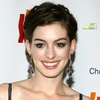
\includegraphics[width=0.3\linewidth]{AH.jpg}
& 
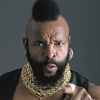
\includegraphics[width=0.3\linewidth]{MrT.jpg}
\end{tabular}
\caption{Deux images des 2 classes à discriminer. À gauche : label 0 (20$\sim$26 ans), et à droite : label 1 (52$\sim$62 ans).}
\end{figure}

$\Rightarrow$ \textbf{Un compte-rendu est à rendre à la fin des 4 heures de TP ou au plus tard une semaine après le TP (notations distinctes dans ces deux cas de figures).}

\section{Questions}

\noindent 1) Décrivez la structure du réseau de neurones utilisé pour l'entraînement. Quel est le nombre total de paramètres de ce réseau ? Détailler la réponse. 
\newline

\noindent 2) Montrez que le réseau initialisé ne classifie pas mieux qu'un choix aléatoire.
\newline

\noindent 3) Préparez le code de façon à enregistrer une courbe d'apprentissage pendant l'entraînement (c'est-à-dire la progression de la performance en fonction du nombre d'itérations). La courbe sera à insérer dans le compte-rendu.
\newline

\noindent 4) Effectuez l'entraînement du réseau (viser une performance supérieure à 75 \%, qui pourra être améliorée continuellement pendant les 4 heures du TP). Indiquez l'accuracy finale obtenue.
\newline

\noindent 5) Évaluez les résultats obtenus avec des mesures 
plus informatives que la simple "accuracy". Pour une classe donnée, on pourra par exemple
mesurer la moyenne et la variance des différences entre les estimation de probabilité de chaque label. Illustrez également vos résultats.
\newline

\noindent 6) Donnez une liste d'hyperparamètres qui pourraient avoir un impact important sur l'entraînement, et expliquez leurs effets.
\newline

\noindent 7) À quoi sert l'utilisation de la fonction \texttt{transforms.RandomCrop()} ?
Remarque : on peut observer les transformations appliquées aux images en utilisant \texttt{original=False} dans les appels à la fonction \texttt{plotdata()}.
\newline

\noindent 8) Mettez au point une procédure où plusieurs "crops" aléatoires sont utilisés pour évaluer la classe d'une image de visage. Vérifiez que cela améliore les performances de classification.
\newline

\noindent 9) Cherchez des images de l'ensemble de données sur lesquelles le réseau entraîné se trompe complètement. Expliquez la procédure mise en place. Cherchez également le contraire : les images sur lesquelles le réseau se trompe le moins.
\newline

\noindent 10) Généralisation hors de la base de données d'entraînement et de test : collectez (sur internet par exemple) une vingtaine d'images de visages centrées et ajustées de manière similaire à celles de la base de donnée, et testez le réseau entraîné pour vérifier qu'il fonctionne correctement.
\newline

\noindent 11) Après vous être renseigné$\cdot$e$\cdot$s sur la méthode appelée "CycleGAN", décrivez comment cette dernière pourrait être appliquée afin d'entraîner un réseau à artificiellement vieillir ou rajeunir une image de visage.
\newline 

\noindent 12) (\emph{Question subsidiaire}) Optimisation des entrées : comment feriez-vous pour construire une image d'entrée qui maximise le résultat de la classification par le réseau (par exemple en maximisant la probabilité estimée que le label soit 0) ? Si vous avez le temps, essayez de mettre cette méthode en oeuvre.

\end{document}

